% !TEX encoding = UTF-8 Unicode

\documentclass[twocolumn,10pt,a4j]{ltjsarticle}
\usepackage{kougai}

\title{ゲームに最適化されたベンチマークソフト「FlexBench」開発}
\author{2032087 大司 陽輝  指導教員 須田 宇宙 准教授}
\date{}

\begin{document}

\maketitle

\section{はじめに}

ゲームに注目が集まりゲームが快適に行えるパソコン(ゲーミングパソコン)の需要が増加している.
しかし,ゲームが快適に行えるパソコンを選ぶには専門の知識が必要となる.
それに対して,ベンチマークソフトを使うことで,ゲームに対してパソコンがスムーズに動作するかの快適度を知る事ができる.
ここでいう快適度は、アイテムなどの境目が鮮明に判断でき、文字の粗や色ずれが起きない程度とし、操作に遅延を感じないことを指標とする。

しかし,ゲームタイトルごとに,必要となるパソコンの性能や, 画質やスムーズさなどの求められる要件が異なる,
また,同じゲームの動作でも開発者によってパソコンの性能の使い方が異なるため,
既存のベンチマークソフトでは,ゲームがどれだけ快適に動作するかを知るには不十分な点がある.
そこで,本研究では,画質などを変更することで,ゲームの負荷を再現し,ゲームごとにどれだけ快適に動作するかを知る事ができるベンチマークソフトを目的とする.

\section{ベンチマークについて}
ゲームでは、物体などの物理演算やシナリオの進行、キャラクターの動作の決定、それらの描画、BGMの再生やスコアの計算が行われている.
これらを,実時間で処理するために,演算の簡略化や並列処理化(マルチスレッド化),別のパーツへの処理の分散が行われているが,その実現方法はゲームタイトルごとに異なる.

また、パソコンのパーツの構成によっては,高い描画力に対応できるものもあれば,スムーズに動作することに重きを置いたものもあり,
高い描画力を必要とするゲームでは,映像を処理するパーツが重要視され、銃撃戦などのゲームではより速いレスポンスが求められる.

その上で,パソコンのゲーム性能を測定しようとしても,ゲームタイトルごとに処理の仕方が異なり,それに従ってパソコンのパーツごとの要求されるスペックが異なる.
%一方,ハードウェア面のパソコン本体の構成としては、同じ金額のパソコンでもそれぞれのパーツに割り振るパーツの金額も異なり、組み合わせとして無数にある。
現状パソコンのゲーム性能を測定するベンチマークソフトが存在するが,描画性能に重きが置かれているので大雑把な性能しか測定できない

\section{FlexBenchについて}
そこで本研究では,ゲームタイトルごとの演算内容などを模擬した上で調整機能を付けることで,実際のゲーム性能を測れると考えた.
開発環境はUnityを使用する.実際に開発したソフトでは,実際にプレイしたゲームの負荷を再現し,プリセットの調整を行う.




\begin{figure}[h]
\begin{center}
 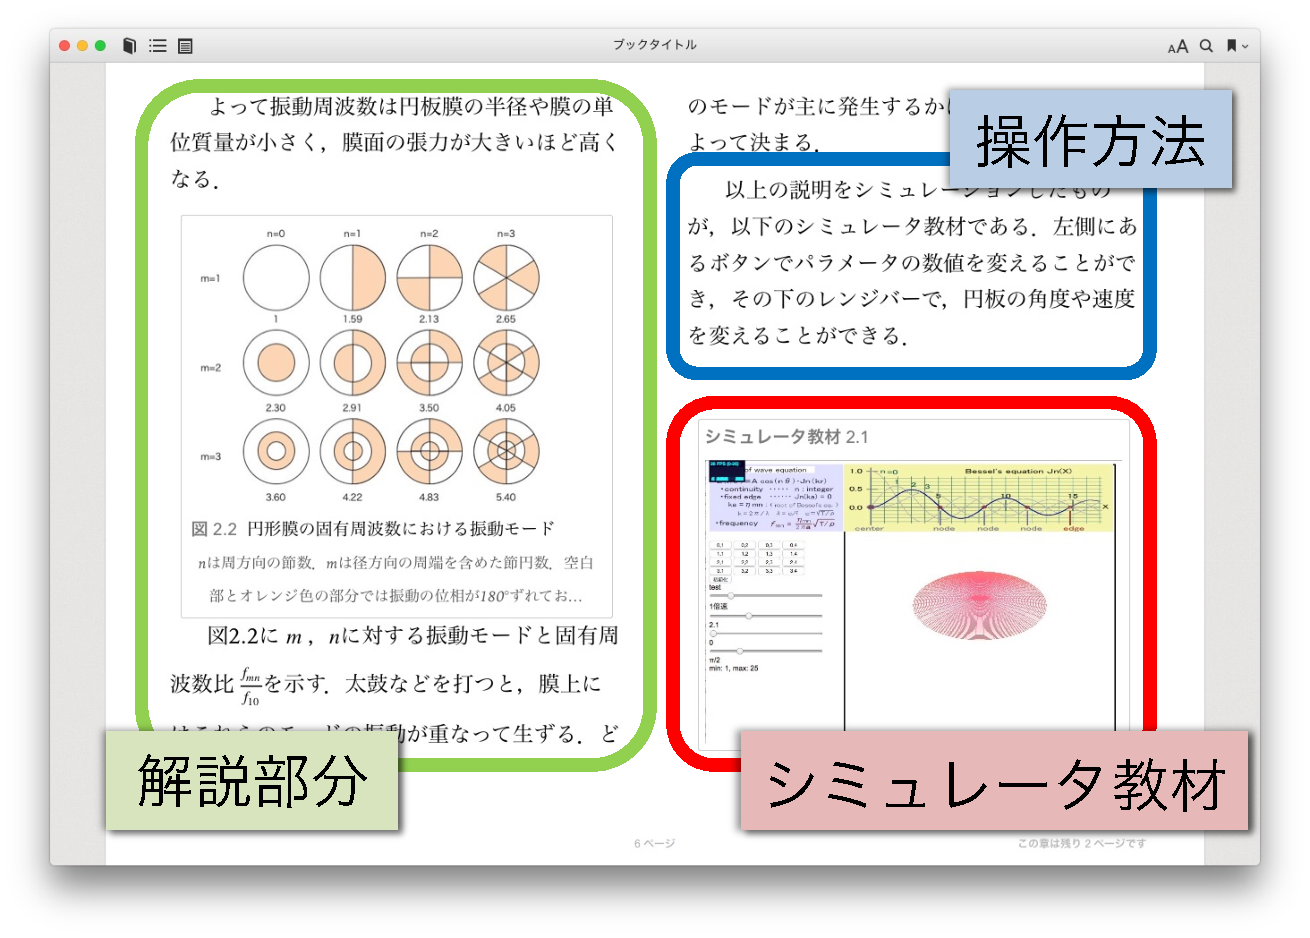
\includegraphics[clip,width=85mm,height=55mm]{textbook.pdf}
\end{center}
 \caption{電子教科書サンプル}
 \label{fig:教科書}
\end{figure}

\section{やること・やったこと}

論文や書籍から,ゲームで行われるグラフィックなどの処理を学び,開発を行うベンチマークソフトの参考とする.


\section{今後の予定}
Unityで,ゲームと同様の処理を行えるソフトの開発を行う

\begin{thebibliography}{99}
\bibitem{1} 須田宇宙: ``音響科学e-Learning教材'', \url{https://www.youtube.com/watch?v=rZdvL0ju4CA&ab_channel=TheSpyHood}, 2018/7/19参照
\end{thebibliography}

\end{document}
